\documentclass[11pt,reqno]{amsart}

\usepackage[T1]{fontenc}
\usepackage{lmodern}
\usepackage[utf8]{inputenc}
\usepackage{amsmath,amssymb,amsthm,mathtools}
\usepackage{booktabs,array,multirow}
\usepackage{graphicx}
\usepackage[margin=1.1in]{geometry}
\usepackage{microtype}
\emergencystretch=1.5em
\usepackage{enumitem}
\usepackage{xcolor}
\definecolor{linkblue}{RGB}{0,51,102}
\definecolor{citeburgundy}{RGB}{128,0,32}
\usepackage[colorlinks=true,linkcolor=linkblue,citecolor=citeburgundy,urlcolor=linkblue]{hyperref}

\newtheorem{theorem}{Theorem}[section]
\newtheorem{proposition}[theorem]{Proposition}
\newtheorem{lemma}[theorem]{Lemma}
\newtheorem{corollary}[theorem]{Corollary}
\theoremstyle{definition}
\newtheorem{definition}[theorem]{Definition}
\theoremstyle{remark}
\newtheorem{remark}[theorem]{Remark}

\numberwithin{equation}{section}

\newcommand{\R}{\mathbb{R}}
\newcommand{\C}{\mathbb{C}}
\newcommand{\Z}{\mathbb{Z}}
\newcommand{\N}{\mathbb{N}}
\newcommand{\dd}{\mathrm{d}}
\newcommand{\ii}{\mathrm{i}}
\newcommand{\ee}{\mathrm{e}}
\DeclareMathOperator{\Reop}{Re}
\DeclareMathOperator{\Imop}{Im}
\DeclareMathOperator{\sgn}{sgn}
\DeclareMathOperator{\sinchyp}{sinc_{hyp}}

\title[Hecke Kernels vs.\ Davenport--Heilbronn Diagnostics]{Hecke Theta-Integral Kernels and Single-Mode Damping in General Degree $L$-Functions versus Off-Line Zero Diagnostics in the Davenport--Heilbronn Counterexample}

\author{Thijs Missiaen}
\address{Independent Researcher, Belgium (ORCID: \href{https://orcid.org/0009-0007-3678-0810}{0009-0007-3678-0810})}
\email{thijs.missiaen@gmail.com}
\date{October 2026}

\subjclass[2020]{Primary 11M41, 11M26; Secondary 11F66, 30D15, 46E22}
\keywords{Selberg class, Davenport--Heilbronn function, Hecke theta-integral, Ramanujan $\Delta$ $L$-function, transverse Wronskian, Euler-product mollifiers, Hadamard--Poisson flux, de Branges kernels}

\begin{document}

\begin{abstract}
Any analytic test for zeros on the critical line must separate $L$-functions with an Euler product from Dirichlet series satisfying a real-even functional equation without an Euler product, notably the Davenport--Heilbronn counterexample $\mathcal{D}_{\mathrm{DH}}(s)$ \cite{davenport1936,titchmarsh1986}. First, we record that Hecke's theta-integral dilation $\varphi_m^{(f)}(u) = a_f(m)m^{-1/2}\varphi_1^{(f)}(u + \frac{1}{2}\ln m)$, asymptotic branch damping $\rho_{\Gamma,f}(d,t)n^{2d} < \ee^{-2d\omega_{n,Q_f}(t)}$, and the single-mode hyperbolic identity $|T_n^{(f)}(d,t)|^2 - |T_n^{(f)}(0,t)|^2 = 4(|a_f(n)|^2/n)\sinh^2(d\omega_{n,Q_f}(t))$ depend solely on the Archimedean functional equation and hold identically for $\zeta(s)$, Ramanujan's $L(s,\Delta)$, and $\mathcal{D}_{\mathrm{DH}}(s)$. Second, we compute the multiplicativity defect $\delta_{\mathrm{DH}}(m,n) = \pm(1+\kappa^2)$ at $N \in \{4,6,9,14\}$: at the first off-line zero $(d_*,\gamma_*) \approx (0.30852, 85.69935)$, prime modes $p \le 7$ supply $38.81780\%$ of $|T_1^{(\mathrm{DH})}|$, non-multiplicative composites $n \in \{4,6,8\}$ supply $54.02700\%$, and the Riemann--Siegel tail $\mathcal{R}_8^{(\mathrm{DH})}$ supplies the remaining $7.25126\%$ residual. Third, we verify four classical zero-detection contrapositives around $(d_*,\gamma_*)$ and clarify why they detect, rather than prevent, off-line zeros.
\end{abstract}

\maketitle

\section{Introduction}
\label{sec:intro}

In Section~10.25 of his treatise on the Riemann zeta-function, Titchmarsh \cite{titchmarsh1986} highlights the classical litmus test introduced by Davenport and Heilbronn \cite{davenport1936}: let $\chi_5$ denote the odd primitive Dirichlet character modulo~$5$ defined by $\chi_5(1)=1$, $\chi_5(2)=\ii$, $\chi_5(3)=-\ii$, $\chi_5(4)=-1$, and $\chi_5(5)=0$, and set
\begin{equation}
  \kappa := \frac{\sqrt{10 - 2\sqrt{5}} - 2}{\sqrt{5} - 1} = 0.284079043840412\ldots,
  \qquad
  \mathcal{D}_{\mathrm{DH}}(s) := \frac{1 - \ii\kappa}{2}\,L(s, \chi_5) + \frac{1 + \ii\kappa}{2}\,L(s, \overline{\chi_5}).
  \label{eq:dh-def}
\end{equation}
Because the Gauss sum of $\chi_5$ is $\tau(\chi_5) = \sum_{a=1}^{4}\chi_5(a)\ee^{2\pi\ii a/5} = -\sqrt{\frac{5 - \sqrt{5}}{2}} + \ii\sqrt{\frac{5 + \sqrt{5}}{2}}$ ($|\tau(\chi_5)| = \sqrt{5}$) with root number $\varepsilon(\chi_5) = \frac{\tau(\chi_5)}{\ii\sqrt{5}} = \frac{1 + \ii\kappa}{1 - \ii\kappa}$, so that $(1 - \ii\kappa)\Lambda(s,\chi_5) = (1 + \ii\kappa)\Lambda(1-s,\overline{\chi_5})$, the completed entire function
\begin{equation}
  \xi_{\mathrm{DH}}(s) := \left(\frac{\pi}{5}\right)^{-(s+1)/2} \Gamma\!\left(\frac{s+1}{2}\right) \mathcal{D}_{\mathrm{DH}}(s),
  \qquad
  \Xi_{\mathrm{DH}}(z) := \xi_{\mathrm{DH}}\!\left(\tfrac{1}{2} + \ii z\right),
  \label{eq:xi-dh-def}
\end{equation}
satisfies the exact real-even functional equation $\xi_{\mathrm{DH}}(s) = \xi_{\mathrm{DH}}(1 - s)$, i.e.\ $\Xi_{\mathrm{DH}}(z) = \Xi_{\mathrm{DH}}(-z) = \overline{\Xi_{\mathrm{DH}}(\bar{z})}$, with real Dirichlet coefficients $a_{\mathrm{DH}}(1)=1$, $a_{\mathrm{DH}}(2)=\kappa$, $a_{\mathrm{DH}}(3)=-\kappa$, $a_{\mathrm{DH}}(4)=-1$, and $a_{\mathrm{DH}}(5)=0$. Yet $\mathcal{D}_{\mathrm{DH}}(s)$ possesses no Euler product, and Davenport and Heilbronn proved that $\mathcal{D}_{\mathrm{DH}}(s)$ has infinitely many zeros in $\Reop(s) > 1$ as well as infinitely many off-critical zeros inside $0 < \Reop(s) < 1$ (see also Spira \cite{spira1994}, Balanzario and S\'anchez-Ortiz \cite{balanzario2007}, and Bombieri and Ghosh \cite{bombieri2011}); its lowest off-line zero in the critical strip occurs at
\begin{equation}
  s_* = \sigma_* + \ii\gamma_* = 0.8085171825\ldots + 85.6993484854\ldots\,\ii,
  \qquad
  d_* := \sigma_* - \tfrac{1}{2} = 0.3085171825\ldots
  \label{eq:dh-first-zero}
\end{equation}

Any analytic program that studies Riemann's $\Xi$-function \cite{riemann1859} through its theta-kernel representation, Wigner phase-space distribution \cite{wigner1932,hudson1974}, Cauchy--Riemann nodal geometry \cite{speiser1934,ariasdereyna2003}, or transverse Wronskian / de~Branges positivity \cite{debranges1968,hinkkanen1997,lagarias1999} must therefore cleanly separate two classes of results:
\begin{enumerate}[label=(\alph*),leftmargin=2.2em]
  \item \emph{Archimedean functional-equation identities}, which hold just as strictly for $\Xi_{\mathrm{DH}}(z)$ as for $\Xi(z)$ and hence cannot by themselves exclude off-line zeros;
  \item \emph{Multiplicative versus non-multiplicative arithmetic features and zero-detection diagnostics}, where $\mathcal{D}_{\mathrm{DH}}(s)$ diverges quantitatively from Selberg-class $L$-functions \cite{selberg1992,kaczorowski1999} and triggers classical positivity contrapositives around $(d_*,\gamma_*)$.
\end{enumerate}

The main results of this paper establish this separation explicitly and quantitatively:

\begin{theorem}[Archimedean invariance, DH multiplicativity defects, and four-layer zero detection]
\label{thm:main-summary}
Let $L(s,f) = \sum_{n=1}^{\infty} a_f(n)n^{-s}$ ($\Reop(s) > 1$) be a self-dual Dirichlet series with Archimedean completion $\xi_f(s) = P_f(s)\mathcal{G}_f(s)L(s,f) = \xi_f(1-s)$ of positive degree $d_f = 2\sum_{j=1}^{r}\lambda_j > 0$, where $\mathcal{G}_f(s) = Q_f^s \prod_{j=1}^{r}\Gamma(\lambda_j s + \mu_j)$. Then:
\begin{enumerate}[label=\textup{(\roman*)},leftmargin=2.3em]
  \item \textbf{Hecke theta-integral dilation and single-mode hyperbolic identity (Sections~\ref{sec:wavelet}--\ref{sec:ellipse}):} Termwise Mellin inversion \cite{hecke1936} expresses the Dirichlet kernel via dilations $\varphi_m^{(f)}(u) = a_f(m)m^{-1/2}\varphi_1^{(f)}(u + \frac{1}{2}\ln m)$ of the single-mode Archimedean profile $\varphi_1^{(f)}(u)$. In the high-frequency regime where $\lambda_j t > \lambda_j(\frac{1}{2}+d)+\Reop\mu_j + 1$ for each $1\le j\le r$, tetragamma positivity ($\Reop\psi_2 > 0$) yields strict branch damping $\rho_{\Gamma,f}(d,t)n^{2d} < \ee^{-2d\omega_{n,Q_f}(t)} \le 1$ for $1 \le n \le N_f(t)$. Moreover, each coupled Riemann--Siegel mode $T_n^{(f)}(d,t)$ satisfies the elementary hyperbolic identity
  \begin{equation}
    \bigl|T_n^{(f)}(d,t)\bigr|^2 - \bigl|T_n^{(f)}(0,t)\bigr|^2
    = 4\,\frac{|a_f(n)|^2}{n}\,\sinh^2\bigl(d\,\omega_{n,Q_f}(t)\bigr) \ge 0.
    \label{eq:intro-ellipse}
  \end{equation}
  All three properties hold identically for $\zeta(s)$ ($d_\zeta = 1$), Ramanujan's modular $L$-function $L(s,\Delta)$ ($d_\Delta = 2$), and $\mathcal{D}_{\mathrm{DH}}(s)$ ($d_{\mathrm{DH}} = 1$).
  \item \textbf{Multiplicativity defect and 8-mode vector anatomy in $\mathcal{D}_{\mathrm{DH}}(s)$ (Section~\ref{sec:prime-gauge}):} On $\Reop(s) > 1$, multiplying an Euler-product $L$-function by the finite prime-factor polynomial $E_X^{(f)}(s) = \prod_{p\le X}P_p^{(f)}(p^{-s})$ \cite{gonek2007} annihilates all composite coefficients on $2\le N\le X$ and restricts $(X,X^2]$ to prime powers. By contrast, $\mathcal{D}_{\mathrm{DH}}(s)$ violates multiplicativity by
  \begin{equation}
    \delta_{\mathrm{DH}}(m,n) := a_{\mathrm{DH}}(mn) - a_{\mathrm{DH}}(m)a_{\mathrm{DH}}(n) = \pm(1 + \kappa^2) = \pm 1.0807009032\ldots
    \label{eq:intro-defect}
  \end{equation}
  at $N \in \{4,6,9,14\}$. While $\zeta(s)$ and $\mathcal{D}_{\mathrm{DH}}(s)$ both have unit-modulus composite coefficients $|a(4)|=|a(6)|=1$, $\mathcal{D}_{\mathrm{DH}}(s)$ has suppressed prime coefficients $|a_{\mathrm{DH}}(2)|=|a_{\mathrm{DH}}(3)|=\kappa \approx 0.28408$, amplifying $|a_{\mathrm{DH}}(4)|/\kappa^2 \approx 12.39143$ relative to multiplicative scaling. At $(d_*,\gamma_*)$ with $N_5(\gamma_*)=8$, prime modes $p\in\{2,3,5,7\}$ provide $38.81780\%$ of $|T_1^{(\mathrm{DH})}|$, composite modes $n\in\{4,6,8\}$ provide $54.02700\%$, and the truncated 8-mode sum retains a non-zero residual $|T_{1..8}^{(\mathrm{DH})}(d_*,\gamma_*)| = 0.17345$ ($7.25126\%$ of $|T_1^{(\mathrm{DH})}|$), cancelled only by the Riemann--Siegel remainder $\mathcal{R}_8^{(\mathrm{DH})}$.
  \item \textbf{Four-layer off-line zero detection (Section~\ref{sec:diagnostics}):} Around $(d_*,\gamma_*)$, $\Xi_{\mathrm{DH}}$ triggers four simultaneous contrapositives of classical critical-line equivalences: (1) a critical-line Laguerre defect $c_1^{\mathrm{DH}}(z_{\mathrm{c}}) < 0$ at $z_{\mathrm{c}} = 85.7472008265$ \cite{jensen1913,csordas1994} with reversed nodal-wall modulus derivative $\dd|R_{\mathrm{DH}}|/\dd s = -|\nabla I_{\mathrm{DH}}| < 0$; (2) negative reduced Wronskian $\widetilde{W}_{\mathrm{DH}}(d,\gamma_*) < 0$ on $[0,d_*)$ \cite{hinkkanen1997,lagarias1999}; (3) a quantized Poisson--Hadamard flux jump $\pi\,\Theta(d - d_*)$; and (4) a Sylvester signature jump $\nu_- : 0 \to 1$ in Pick--Nevanlinna matrices of $\Theta_\alpha^{\mathrm{DH}}$ \cite{debranges1968}. These four signatures constitute exact zero-detection diagnostics rather than a zero-prevention proof.
\end{enumerate}
\end{theorem}

\subsection{Proof overview}
\label{subsec:proof-overview}

Section~\ref{sec:wavelet} derives the Hecke theta-integral representation for general Archimedean factors $\mathcal{G}_f(s)$ via Mellin inversion on $\Reop(s) > 1$ and proves strict branch damping using the sign of the real part of the tetragamma function $\psi_2(w) = \psi''(w)$ in the high-frequency regime $|\Imop w| > \Reop w > 0$. Section~\ref{sec:ellipse} verifies the elementary hyperbolic-trigonometric ellipse identity for general complex coefficients $a_f(n)$ and tabulates all $N_5(\gamma_*) = 8$ modes of $\Xi_{\mathrm{DH}}$ at $(d_*,\gamma_*)$. Section~\ref{sec:prime-gauge} compares Euler-product mollification on $\Reop(s) > 1$ against the exact trigonometric identity $\sin(\theta_5 + \alpha)\sin(\theta_5 + \beta) - \cos\theta_5\sin(\theta_5 + \alpha + \beta) = -\sin\alpha\sin\beta$ underlying $\delta_{\mathrm{DH}}(m,n) = \pm(1+\kappa^2)$, and establishes the complete complex vector balance $T_1^{(\mathrm{DH})} + \sum_{p\le 7}T_p^{(\mathrm{DH})} + \sum_{n\in\{4,6,8\}}T_n^{(\mathrm{DH})} + \mathcal{R}_8^{(\mathrm{DH})} = 0$. Section~\ref{sec:diagnostics} evaluates all four zero-detection contrapositives around $(d_*,\gamma_*)$. Section~\ref{sec:scope} records the scope, limitations, and structural obstructions, including why single-mode damping and zero-detection equivalences do not prevent off-line zeros. Appendix~\ref{app:interval} documents the 60-decimal and 35-decimal interval-arithmetic verification protocol.

\subsection{Notation and conventions}
\label{subsec:notation}

Throughout, $s = \sigma + \ii t = \frac{1}{2} + d + \ii t$ with transverse coordinate $d = \sigma - \frac{1}{2} \ge 0$ and spectral parameter $z = t - \ii d$, so $\frac{1}{2} + \ii z = \frac{1}{2} + d + \ii t$. For any real-even entire completion $\Xi_f(z) = \xi_f(\frac{1}{2}+\ii z)$ written in canonical cosine-transform normalization
\begin{equation}
  \Xi_f(z) = 8 \int_{0}^{\infty} \Phi_f(u)\cos(2zu)\,\dd u,
  \qquad
  \Xi_f(t - \ii d) = R_f(d,t) + \ii I_f(d,t),
  \label{eq:canonical-xi}
\end{equation}
where $\Phi_f(-u) = \Phi_f(u)$ is real-even (for $f=\zeta$, $\Phi_\zeta(u) = \sum_{n=1}^{\infty}(2\pi^2 n^4 \ee^{9u} - 3\pi n^2 \ee^{5u})\ee^{-\pi n^2 \ee^{4u}}$ is Riemann's Jacobi-theta kernel \cite{riemann1859,polya1926}), the canonical transverse Wronskian and its Wigner phase-space representation \cite{wigner1932,hudson1974} are defined by
\begin{align}
  W_f(d,t) &:= \frac{1}{2}\,\partial_d\bigl|\Xi_f(t - \ii d)\bigr|^2
  = R_f\,\partial_d R_f + I_f\,\partial_d I_f
  = R_f\,\partial_t I_f - I_f\,\partial_t R_f \nonumber\\
  &= 16 \int_{0}^{\infty} y\sinh(2dy)\,I_f(y,t)\,\dd y,
  \label{eq:canonical-wronskian}
\end{align}
where $I_f(y,t) := 2\int_{0}^{\infty}\Phi_f\!\left(\frac{y+r}{2}\right)\Phi_f\!\left(\frac{y-r}{2}\right)\cos(2tr)\,\dd r$. The parity-reduced Wronskian is $\widetilde{W}_f(d,t) := W_f(d,t)/d = 32\int_{0}^{\infty}y^2\sinchyp(2dy)\,I_f(y,t)\,\dd y$, with $\sinchyp(x) := \sinh(x)/x$ ($\sinchyp(0):=1$) and critical-line limit $c_1^f(t) := \widetilde{W}_f(0,t) = (\Xi_f'(t))^2 - \Xi_f(t)\Xi_f''(t)$. Here $\psi(w) = \Gamma'(w)/\Gamma(w)$ denotes the digamma function, $\psi_k(w) := \psi^{(k)}(w)$ the polygamma functions, $\vartheta_f(t) := \arg\mathcal{G}_f(\frac{1}{2}+\ii t)$, and $\omega_{n,Q_f}(t) := \vartheta_f'(t) - \ln n$ the local mode saddle velocity with cutoff $N_f(t) := \lfloor \ee^{\vartheta_f'(t)} \rfloor$.

\section{Hecke Theta-Integral Dilation and Asymptotic Branch Damping}
\label{sec:wavelet}

We begin by recording Hecke's classical Mellin--theta representation \cite{hecke1936} in logarithmic dilation coordinates $u \in \R$ and verifying the exact high-frequency branch-damping inequality across degree-$d_f$ Archimedean completions.

\begin{theorem}[Hecke dilation and tetragamma damping]
\label{thm:mother-wavelet}
Let $L(s,f) = \sum_{n=1}^{\infty} a_f(n)n^{-s}$ converge absolutely on $\Reop(s) > 1$. Suppose its self-dual completion is $\xi_f(s) = P_f(s)\mathcal{G}_f(s)L(s,f) = \xi_f(1-s)$ with $\mathcal{G}_f(s) = Q_f^s\prod_{j=1}^{r}\Gamma(\lambda_j s + \mu_j)$, $\lambda_j > 0$, $\Reop(\frac{1}{2}\lambda_j + \mu_j) > 0$, $\{\mu_j\} = \{\overline{\mu_j}\}$ as multisets, and real-symmetric polynomial $P_f(s) = P_f(1-s)$ annihilating any polar singularities. Define the single-mode inverse Mellin profile
\begin{equation}
  \varphi_1^{(f)}(u) := \frac{1}{\pi}\int_{-\infty}^{\infty} P_f\!\left(\tfrac{1}{2} + \ii\tau\right)\mathcal{G}_f\!\left(\tfrac{1}{2} + \ii\tau\right)\ee^{-2\ii\tau u}\,\dd\tau
  \qquad (u \in \R).
  \label{eq:mother-wavelet-def}
\end{equation}
Then:
\begin{enumerate}[label=\textup{(\roman*)},leftmargin=2.2em]
  \item \textbf{Dilation and symmetry:} By Stirling's decay $|\mathcal{G}_f(\frac{1}{2}+\ii\tau)| \ll (1+|\tau|)^A \ee^{-\frac{\pi}{4}d_f|\tau|}$, $\varphi_1^{(f)}$ extends holomorphically to $|\Imop u| < \frac{\pi}{8}d_f$ with super-exponential real-axis decay. For $\Reop(\frac{1}{2}+\ii z) > 1$, Mellin inversion gives $\Xi_f(z) = 8\int_0^\infty \Phi_f(u)\cos(2zu)\,\dd u$ with $\Phi_f(u) = \frac{1}{8}(\widetilde{\Phi}_f(u) + \widetilde{\Phi}_f(-u)) + \Phi_{f,\mathrm{pole}}(u)$, where each mode $m\ge 1$ is a pure shift-dilation of $\varphi_1^{(f)}$:
  \begin{equation}
    \boxed{
    \widetilde{\Phi}_f(u) = \sum_{m=1}^{\infty} \varphi_m^{(f)}(u),
    \qquad
    \varphi_m^{(f)}(u) \equiv \frac{a_f(m)}{\sqrt{m}}\,\varphi_1^{(f)}\!\left(u + \tfrac{1}{2}\ln m\right).
    }
    \label{eq:boxed-mother-wavelet}
  \end{equation}
  \item \textbf{High-frequency symmetric branch damping:} Let $\rho_{\Gamma,f}(d,t) := |\mathcal{G}_f(\frac{1}{2}-d-\ii t)/\mathcal{G}_f(\frac{1}{2}+d+\ii t)|$. Fix $d > 0$ with $\Reop(\lambda_j(\frac{1}{2}-d)+\mu_j) > 0$ for all $1\le j\le r$, and suppose $t > 0$ satisfies $\lambda_j t > \lambda_j(\frac{1}{2}+d) + |\Reop\mu_j| + 1$ for every $1\le j\le r$. Then
  \begin{equation}
    \rho_{\Gamma,f}(d,t) < \ee^{-2d\,\vartheta_f'(t)},
    \qquad\text{and hence}\qquad
    \rho_{\Gamma,f}(d,t)\,n^{2d} < \ee^{-2d\,\omega_{n,Q_f}(t)} \le 1
    \quad \forall\,1 \le n \le N_f(t).
    \label{eq:branch-damping}
  \end{equation}
\end{enumerate}
\end{theorem}

\begin{proof}
For~(i), shifting the vertical Mellin contour $\Reop(s) = \sigma_0 > 1$ to $\Reop(s) = \frac{1}{2}$ (collecting any finite-order pole residues of $\xi_f$ into $\Phi_{f,\mathrm{pole}}(u)$) and substituting $s = \frac{1}{2} + \ii\tau$ expresses the $m$-th Dirichlet term $a_f(m)m^{-(\frac{1}{2}+\ii\tau)} = a_f(m)m^{-1/2}\ee^{-\ii\tau\ln m}$ as a Fourier shift $2u \mapsto 2u + \ln m$ inside~\eqref{eq:mother-wavelet-def}, yielding~\eqref{eq:boxed-mother-wavelet}; functional-equation symmetry $\xi_f(1-s)=\xi_f(s)$ then ensures $\Phi_f(-u)=\Phi_f(u)$ upon Poisson summation \cite{hecke1936}. Explicit closed forms for $\zeta(s)$, $L(s,\chi_5)$ (hence $\mathcal{D}_{\mathrm{DH}}(s)$), and Ramanujan's weight-$12$ cusp form $L(s,\Delta)$ ($d_\Delta = 2$, normalized at $s \mapsto s + \frac{11}{2}$):
\begin{align}
  \varphi_1^{(\zeta)}(u) &= 4\pi^2 \ee^{9u}\ee^{-\pi\ee^{4u}} - 6\pi\ee^{5u}\ee^{-\pi\ee^{4u}}, &
  \varphi_1^{(\mathrm{odd},5)}(u) &= 2\,\ee^{3u}\,\ee^{-\frac{\pi}{5}\ee^{4u}}, &
  \varphi_1^{(\Delta)}(u) &= \frac{1}{2}\,\ee^{12u}\,\ee^{-2\pi\ee^{2u}},
  \label{eq:explicit-mother-wavelets}
\end{align}
follow directly from Cahen--Mellin inversion $\frac{1}{2\pi\ii}\int_{(c)}\Gamma(w)x^{-w}\,\dd w = \ee^{-x}$.

For~(ii), set $g(u) := \ln|\mathcal{G}_f(\frac{1}{2}+u+\ii t)|$. Since $\{\mu_j\}=\{\overline{\mu_j}\}$ implies $|\mathcal{G}_f(\bar{s})| = |\mathcal{G}_f(s)|$, we have
\begin{equation}
  \rho_{\Gamma,f}(d,t) = \exp\bigl(-\bigl[g(d) - g(-d)\bigr]\bigr)
  = \exp\!\left(-\int_{0}^{d} \mathcal{A}_{\Gamma,f}^{\mathrm{sym}}(u,t)\,\dd u\right),
  \label{eq:rho-integral}
\end{equation}
where $\mathcal{A}_{\Gamma,f}^{\mathrm{sym}}(u,t) := g'(u) + g'(-u) = 2\ln Q_f + \sum_{j=1}^{r}\lambda_j\bigl[\Reop\psi(\lambda_j(\frac{1}{2}+u+\ii t)+\mu_j) + \Reop\psi(\lambda_j(\frac{1}{2}-u+\ii t)+\overline{\mu_j})\bigr]$. Notice that $\mathcal{A}_{\Gamma,f}^{\mathrm{sym}}(u,t)$ is smooth and \emph{even} in $u$, with $\mathcal{A}_{\Gamma,f}^{\mathrm{sym}}(0,t) = 2\vartheta_f'(t)$ by Cauchy--Riemann differentiation $\vartheta_f'(t) = \partial_t\Imop\ln\mathcal{G}_f(\frac{1}{2}+\ii t) = g'(0)$, and $\partial_u\mathcal{A}_{\Gamma,f}^{\mathrm{sym}}(0,t) = g''(0) - g''(0) = 0$. Differentiating \emph{twice} with respect to~$u$ gives
\begin{equation}
  \partial_u^2 \mathcal{A}_{\Gamma,f}^{\mathrm{sym}}(u,t)
  = g'''(u) + g'''(-u)
  = \sum_{j=1}^{r}\lambda_j^3\Bigl[\Reop\psi_2\bigl(w_j^+(u)\bigr) + \Reop\psi_2\bigl(w_j^-(u)\bigr)\Bigr],
  \label{eq:tetragamma-second-deriv}
\end{equation}
where $w_j^{\pm}(u) = \sigma_j^{\pm}(u) + \ii\tau_j^{\pm}$ has $\tau_j^{\pm} = \lambda_j t \pm \Imop\mu_j$ and $0 < \sigma_j^{\pm}(u) = \lambda_j(\frac{1}{2}\pm u) + \Reop\mu_j$. Using the integral representation $\psi_2(w) = -\int_0^\infty v^2 \ee^{-wv}(1 - \ee^{-v})^{-1}\,\dd v$ and Euler--Maclaurin / Binet remainder bounds $\psi_2(w) = -w^{-2} - w^{-3} - \frac{1}{2}w^{-4} + R_2(w)$ with $|R_2(w)| \le \frac{1}{6}|w|^{-5}$ in $\Reop w > 0$, one has $\Reop(-w^{-2} - w^{-3}) = \frac{\tau^2 - \sigma^2}{(\sigma^2+\tau^2)^2} + \frac{3\sigma\tau^2 - \sigma^3}{(\sigma^2+\tau^2)^3} > 0$ whenever $|\tau| > \sigma + 1 > 1$, which easily dominates $\frac{2}{3}|w|^{-4}$. Hence $\partial_u^2\mathcal{A}_{\Gamma,f}^{\mathrm{sym}}(u,t) > 0$ on $u \in [0,d]$, forcing $\mathcal{A}_{\Gamma,f}^{\mathrm{sym}}(u,t) > 2\vartheta_f'(t)$ on $(0,d]$ and yielding~\eqref{eq:branch-damping} upon multiplying by $n^{2d} = \ee^{2d\ln n}$.
\end{proof}

\begin{remark}[Low-height reversal near $t=0$]
\label{rem:low-height}
In~\eqref{eq:tetragamma-second-deriv}, the governing polygamma derivative is the \emph{tetragamma} function $\psi_2 = \psi''$, not the trigamma function $\psi_1 = \psi'$. On the real axis ($t=0$, $\mu_j\in\R$), $\psi_2(\sigma) = -2\sum_{k=0}^{\infty}(\sigma+k)^{-3} < 0$, so the inequality $\rho_{\Gamma,f}(d,t) < \ee^{-2d\vartheta_f'(t)}$ reverses at $t=0$ and holds strictly only above the low-height crossover $|\tau_j^{\pm}| \gtrsim \sigma_j^{\pm}$ where $\Reop(-w^{-2}) > 0$. At all spectral heights relevant to nontrivial zeros (such as $\gamma_1 \approx 14.13473$ for $\zeta$ and $\gamma_* \approx 85.69935$ for $\mathcal{D}_{\mathrm{DH}}$), the hypothesis of Theorem~\ref{thm:mother-wavelet}(ii) holds with wide margin (Table~\ref{tab:branch-damping}).
\end{remark}

\begin{table}[htbp]
\centering
\caption{Verification of symmetric branch damping $\rho_{\Gamma,f}(d,t) < \ee^{-2d\vartheta_f'(t)}$ across degree-$1$ and degree-$2$ completions at $d = d_* = 0.3085171825$ (certified in \nolinkurl{verify_paper12_selberg_davenport_heilbronn.py}).}
\label{tab:branch-damping}
{\footnotesize\setlength{\tabcolsep}{4pt}%
\begin{tabular}{@{}lcccccc@{}}
\toprule
Completion class & $d_f$ & Height $t$ & $N_f(t)$ & $\rho_{\Gamma,f}(d_*,t)$ & $\ee^{-2d_*\vartheta_f'(t)}$ & Margin $\ee^{-2d_*\vartheta_f'(t)} - \rho_{\Gamma,f}$ \\
\midrule
Riemann $\zeta(s)$ & $1$ & $85.69935$ & $3$ & $0.4465765317$ & $0.4465768293$ & $+2.97605 \times 10^{-7}$ \\
$\mathcal{D}_{\mathrm{DH}}(s)$ / $L(s,\chi_5)$ & $1$ & $85.69935$ & $8$ & $0.2718013692$ & $0.2718015503$ & $+1.81133 \times 10^{-7}$ \\
Ramanujan $L(s,\Delta)$ & $2$ & $25.00000$ & $4$ & $0.4203432003$ & $0.4203489013$ & $+5.70097 \times 10^{-6}$ \\
\bottomrule
\end{tabular}%
}
\end{table}

\section{Single-Mode Hyperbolic Identity Across General Dirichlet Coefficients}
\label{sec:ellipse}

Factoring out the Archimedean envelope $\mathcal{G}_f(\frac{1}{2}+d+\ii t)\ee^{-\ii\vartheta_f(t)}$ in the approximate functional equation produces, for each $1 \le n \le N_f(t)$, the coupled main-sum mode
\begin{equation}
  T_n^{(f)}(d,t) := \frac{a_f(n)}{n^{1/2+d}}\,\ee^{\ii\phi_{n,f}(t)}\,\ee^{d\,\vartheta_f'(t)} + \frac{\overline{a_f(n)}}{n^{1/2-d}}\,\ee^{-\ii\phi_{n,f}(t)}\,\ee^{-d\,\vartheta_f'(t)},
  \label{eq:coupled-mode-def}
\end{equation}
where $\phi_{n,f}(t) := \vartheta_f(t) - t\ln n$. Writing $a_f(n) = |a_f(n)|\ee^{\ii\alpha_n}$ and $\psi_{n,f}(t) := \phi_{n,f}(t) + \alpha_n$ reduces~\eqref{eq:coupled-mode-def} to $T_n^{(f)}(d,t) = 2|a_f(n)|n^{-1/2}[\cosh(d\omega_{n,Q_f}(t))\cos\psi_{n,f}(t) + \ii\sinh(d\omega_{n,Q_f}(t))\sin\psi_{n,f}(t)]$. Applying the elementary Pythagorean and hyperbolic identities $\cos^2\psi + \sin^2\psi = 1$ and $\cosh^2 x - \sinh^2 x = 1$ immediately gives the following proposition.

\begin{proposition}[Single-mode hyperbolic identity and confocal parametrization]
\label{prop:confocal-ellipse}
For every $n \ge 1$, every $d \ge 0$, every $t \in \R$, and arbitrary complex coefficients $a_f(n) \in \C$:
\begin{enumerate}[label=\textup{(\roman*)},leftmargin=2.2em]
  \item \textbf{Phase-independent squared-modulus excess:} Using $T_n^{(f)}(0,t) = 2|a_f(n)|\allowbreak n^{-1/2}\allowbreak\cos\psi_{n,f}(t)$,
  \begin{equation}
    \bigl|T_n^{(f)}(d,t)\bigr|^2 - \bigl|T_n^{(f)}(0,t)\bigr|^2
    = 4\,\frac{|a_f(n)|^2}{n}\,\sinh^2\bigl(d\,\omega_{n,Q_f}(t)\bigr) \ge 0.
    \label{eq:confocal-identity}
  \end{equation}
  \item \textbf{Confocal ellipse geometry:} As $\psi_{n,f}$ varies, $T_n^{(f)}(d,t)$ traces an ellipse with semi-axes $A_n^{(f)} = 2|a_f(n)|n^{-1/2}\cosh(d\omega_{n,Q_f})$ and $B_n^{(f)} = 2|a_f(n)|n^{-1/2}|\sinh(d\omega_{n,Q_f})|$, whose linear focal distance $c_n^{(f)} = \sqrt{(A_n^{(f)})^2 - (B_n^{(f)})^2} = 2|a_f(n)|n^{-1/2}$ is independent of~$d$.
  \item \textbf{Diagonal sum versus off-diagonal interference:} Summing~\eqref{eq:confocal-identity} over $1\le n\le N_f(t)$ makes the diagonal transverse growth $\sum_{n=1}^{N_f(t)} 4(|a_f(n)|^2/n)\sinh^2(d\omega_{n,Q_f}(t))$ strictly positive whenever $a_f(1)=1$ and $N_f(t)\ge 2$.
\end{enumerate}
\end{proposition}

\begin{remark}[Diagonal positivity does not prevent off-line zeros]
\label{rem:diagonal-warning}
Proposition~\ref{prop:confocal-ellipse} illustrates why single-mode hyperbolic growth and diagonal Wronskian positivity can never prove a critical-line theorem on their own: Table~\ref{tab:dh-8modes} confirms that~\eqref{eq:confocal-identity} holds to machine precision for all $N_5(\gamma_*)=8$ modes of $\mathcal{D}_{\mathrm{DH}}(s)$ right at its off-line zero $(d_*,\gamma_*)$. Off-line zeros are governed not by the positive diagonal sum, but by destructive multi-mode cross-term alignment among the $\binom{N_f(t)}{2}$ off-diagonal pairs together with the Riemann--Siegel remainder.
\end{remark}

\begin{table}[htbp]
\centering
\caption{All $N_5(\gamma_*) = 8$ coupled modes of $\mathcal{D}_{\mathrm{DH}}(s)$ at $(d_*, \gamma_*) = (0.3085171825, 85.6993484854)$, verifying~\eqref{eq:confocal-identity} and linear focal distance $c_n^{(\mathrm{DH})} = 2|a_{\mathrm{DH}}(n)|/\sqrt{n}$.}
\label{tab:dh-8modes}
{\footnotesize\setlength{\tabcolsep}{4pt}%
\begin{tabular}{@{}clrrrrr@{}}
\toprule
$n$ & Mode type & $a_{\mathrm{DH}}(n)$ & $\Reop T_n^{(\mathrm{DH})}(d_*,\gamma_*)$ & $\Imop T_n^{(\mathrm{DH})}(d_*,\gamma_*)$ & $|T_n(d_*)|^2 - |T_n(0)|^2$ & $c_n^{(\mathrm{DH})}$ \\
\midrule
$1$ & Leading ($1$) & $+1.00000000$ & $+2.36842317$ & $+0.33461363$ & $1.95095643$ & $2.00000000$ \\
$2$ & Prime ($2$) & $+0.28407904$ & $-0.38035571$ & $-0.09170206$ & $0.03291436$ & $0.40174844$ \\
$3$ & Prime ($3$) & $-0.28407904$ & $-0.32453772$ & $-0.03466788$ & $0.01084736$ & $0.32802622$ \\
$4$ & Composite ($2^2$) & $-1.00000000$ & $-0.70091660$ & $-0.16456287$ & $0.05085699$ & $1.00000000$ \\
$5$ & Ramified ($5$) & $0.00000000$ & $0.00000000$ & $0.00000000$ & $0.00000000$ & $0.00000000$ \\
$6$ & Semiprime ($2\cdot 3$) & $+1.00000000$ & $-0.66424331$ & $-0.04731055$ & $0.00649611$ & $0.81649658$ \\
$7$ & Prime ($7$) & $+0.28407904$ & $-0.21499212$ & $+0.00018520$ & $0.00012002$ & $0.21474357$ \\
$8$ & Composite ($2^3$) & $-0.28407904$ & $+0.09006019$ & $+0.00175934$ & $0.00000387$ & $0.20087422$ \\
\bottomrule
\end{tabular}%
}
\end{table}

\section{Multiplicativity Defects, Mollifier Sieving, and the 8-Mode Vector Balance}
\label{sec:prime-gauge}

We now isolate the precise arithmetic difference between Euler-product $L$-functions and $\mathcal{D}_{\mathrm{DH}}(s)$. First, we emphasize a crucial distinction to avoid a common misconception: an Euler product does \emph{not} make composite Dirichlet coefficients small in absolute value—for $\zeta(s)$, $a_\zeta(4) = a_\zeta(6) = 1$ have the exact same unit modulus as $|a_{\mathrm{DH}}(4)| = |a_{\mathrm{DH}}(6)| = 1$. Rather, Euler-product multiplicativity locks composite coefficients algebraically to products of prime coefficients ($a(mn)=a(m)a(n)$ for $(m,n)=1$), which has two rigorous consequences: (a) under multiplication on $\Reop(s) > 1$ by a finite prime-factor Dirichlet polynomial $E_X^{(f)}(s)$ \cite{gonek2007}, composite modes on $2\le N\le X$ cancel identically; and (b) in $\mathcal{D}_{\mathrm{DH}}(s)$, the prime coefficients at $p=2,3$ have small modulus $|a_{\mathrm{DH}}(2)|=|a_{\mathrm{DH}}(3)|=\kappa \approx 0.28408$, whereas the composite coefficients $a_{\mathrm{DH}}(4)=-1$ and $a_{\mathrm{DH}}(6)=+1$ violate multiplicativity by $\pm(1+\kappa^2)$ and exceed $\kappa^2 \approx 0.08070$ by a factor of $1/\kappa^2 \approx 12.39143$.

\begin{theorem}[Multiplicativity defect, mollifier sieving on $\Reop(s)>1$, and 8-mode vector balance]
\label{thm:prime-gauge-breakdown}
\leavevmode
\begin{enumerate}[label=\textup{(\roman*)},leftmargin=2.2em]
  \item \textbf{Euler-product mollifier sieving on $\Reop(s) > 1$:} Let $L(s,f) = \prod_p P_p^{(f)}(p^{-s})^{-1}$ converge absolutely on $\Reop(s) > 1$, where $P_p^{(f)}(z) = \prod_{i=1}^{d_f}(1 - \alpha_{p,i}z)$. Multiplying $L(s,f)$ by the entire Dirichlet polynomial $E_X^{(f)}(s) := \prod_{p \le X} P_p^{(f)}(p^{-s})$ gives $L(s,f)E_X^{(f)}(s) = \prod_{p>X} P_p^{(f)}(p^{-s})^{-1} = \sum_{N=1}^{\infty} b_N^{(f)}(X)N^{-s}$ ($\Reop(s) > 1$), where $b_1^{(f)}(X) = 1$, $b_N^{(f)}(X) = 0$ for $2 \le N \le X$, and on $(X,X^2]$ the coefficients $b_N^{(f)}(X)$ vanish at every composite $N = pq$ with distinct primes $p,q \le X$ (leaving only primes $p \in (X,X^2]$ and prime powers $p^k$ with $p > X$, or under the formal truncated exponential polynomial $\exp(-\sum_{p^k \le X} \frac{\Lambda_f(p^k)}{k\ln p}p^{-ks})$ on $\Reop(s)>1$, prime powers on $(X,X^2]$).
  \item \textbf{Exact multiplicativity defect in $\mathcal{D}_{\mathrm{DH}}(s)$:} Writing $a_{\mathrm{DH}}(n) = \frac{\Reop[\ee^{-\ii\theta_5}\chi_5(n)]}{\cos\theta_5}$ with $\kappa = \tan\theta_5$, every pair $m,n \ge 2$ satisfies $\delta_{\mathrm{DH}}(m,n) := a_{\mathrm{DH}}(mn) - a_{\mathrm{DH}}(m)a_{\mathrm{DH}}(n)$ with
  \begin{equation}
    \delta_{\mathrm{DH}}(2,2) = -(1 + \kappa^2), \quad
    \delta_{\mathrm{DH}}(2,3) = +(1 + \kappa^2), \quad
    \delta_{\mathrm{DH}}(3,3) = -(1 + \kappa^2), \quad
    \delta_{\mathrm{DH}}(2,7) = -(1 + \kappa^2),
    \label{eq:exact-dh-defects}
  \end{equation}
  where $1 + \kappa^2 = \sec^2\theta_5 = 1.0807009032\ldots$ Consequently, multiplying $\mathcal{D}_{\mathrm{DH}}(s)$ on $\Reop(s)>1$ by $\prod_{p\le 5}(1 - a_{\mathrm{DH}}(p)p^{-s})$ fails to clear $2\le N\le 5$ and $(5,25]$, leaving $b_4^{\mathrm{Euler}}(5) = -(1+\kappa^2)$ and $b_6^{\mathrm{Euler}}(5) = +(1+\kappa^2)$ (and formal Dirichlet logarithm coefficient $\Lambda_{\mathrm{DH}}(6)/\ln 6 = +(1+\kappa^2)$ on $\Reop(s) > 1$).
  \item \textbf{Complete 8-mode and remainder balance at $(d_*,\gamma_*)$:} At $(d_*,\gamma_*) = (0.3085171825,\allowbreak 85.6993484854)$ with $N_5(\gamma_*) = 8$, let $\mathcal{R}_8^{(\mathrm{DH})} := -T_{1..8}^{(\mathrm{DH})}(d_*,\gamma_*)$ denote the exact Riemann--Siegel remainder closing $T_1^{(\mathrm{DH})} + \sum_{p\le 7} T_p^{(\mathrm{DH})} + \sum_{n\in\{4,6,8\}} T_n^{(\mathrm{DH})} + \mathcal{R}_8^{(\mathrm{DH})} = 0$. Then:
  \begin{align}
    \bigl|T_1^{(\mathrm{DH})}\bigr| &= 2.3919436882, \nonumber\\
    \Bigl|\sum_{p \in \{2,3,5,7\}} T_p^{(\mathrm{DH})}\Bigr| &= 0.9284998761 \quad (38.81780\%\text{ of }|T_1^{(\mathrm{DH})}|), \nonumber\\
    \Bigl|\sum_{n \in \{4,6,8\}} T_n^{(\mathrm{DH})}\Bigr| &= 1.2922953320 \quad (54.02700\%\text{ of }|T_1^{(\mathrm{DH})}|), \nonumber\\
    \bigl|\mathcal{R}_8^{(\mathrm{DH})}\bigr| = \bigl|T_{1..8}^{(\mathrm{DH})}\bigr| &= 0.1734460872 \quad (7.25126\%\text{ of }|T_1^{(\mathrm{DH})}|).
    \label{eq:mode-cancellation-anatomy}
  \end{align}
  Replacing $a_{\mathrm{DH}}(n)$ on $n\in\{4,6,8\}$ by multiplicative values $a_{\mathrm{mult}}(4)=\kappa^2$, $a_{\mathrm{mult}}(6)=-\kappa^2$, $a_{\mathrm{mult}}(8)=\kappa^3$ shrinks the composite sum to $0.1042894004$ ($4.36003\%$ of $|T_1^{(\mathrm{DH})}|$) and leaves $|T_{1..8}^{\mathrm{mult}}(d_*,\gamma_*)| = 1.5677252586 \gg |\mathcal{R}_8^{(\mathrm{DH})}|$.
\end{enumerate}
\end{theorem}

\begin{proof}
Part~(i) is immediate on the half-plane of absolute convergence $\Reop(s) > 1$ by cancelling local factors $P_p^{(f)}(p^{-s})$ for $p \le X$; note that while $E_X^{(f)}(s)$ is a finite Dirichlet polynomial (hence entire in~$s$), the infinite reciprocal $\prod_{p>X} P_p^{(f)}(p^{-s})^{-1}$ converges absolutely only on $\Reop(s) > 1$ and requires analytic continuation to reach $0 < \Reop(s) \le 1$.

For~(ii), write $\chi_5(2) = \ee^{\ii\pi/2}$, $\chi_5(3) = \ee^{-\ii\pi/2}$, $\chi_5(4) = -1$, $\chi_5(6) = +1$, $\chi_5(7) = \ee^{\ii\pi/2}$, $\chi_5(9) = -1$, $\chi_5(14) = -1$. Since $a_{\mathrm{DH}}(2) = \tan\theta_5 = \kappa$ and $a_{\mathrm{DH}}(3) = -\kappa$, one computes directly: $\delta_{\mathrm{DH}}(2,2) = -1 - \kappa^2 = -(1+\kappa^2)$, $\delta_{\mathrm{DH}}(2,3) = 1 - (-\kappa^2) = +(1+\kappa^2)$, $\delta_{\mathrm{DH}}(3,3) = -1 - \kappa^2 = -(1+\kappa^2)$, and $\delta_{\mathrm{DH}}(2,7) = -1 - \kappa^2 = -(1+\kappa^2)$. Expanding $\mathcal{D}_{\mathrm{DH}}(s)(1 - \kappa 2^{-s} + \kappa 3^{-s} - \kappa^2 6^{-s})$ on $\Reop(s) > 1$, the factor $1 - \kappa 2^{-s}$ contributes $-\kappa a_{\mathrm{DH}}(2) = -\kappa^2$ at $N=4$, giving $b_4^{\mathrm{Euler}}(5) = a_{\mathrm{DH}}(4) - \kappa a_{\mathrm{DH}}(2) = -(1+\kappa^2)$ and $b_6^{\mathrm{Euler}}(5) = a_{\mathrm{DH}}(6) - \kappa a_{\mathrm{DH}}(3) + \kappa a_{\mathrm{DH}}(2) - \kappa^2 a_{\mathrm{DH}}(1) = +(1+\kappa^2)$.

For~(iii), summing the certified 60-decimal entries in Table~\ref{tab:dh-8modes} yields~\eqref{eq:mode-cancellation-anatomy}. Crucially, $38.81780\% + 54.02700\% = 92.84480\% < 100\%$: the 8-mode main sum $T_{1..8}^{(\mathrm{DH})}(d_*,\gamma_*)$ does not vanish by itself, leaving a residual of $7.25126\%$ of $|T_1^{(\mathrm{DH})}|$ that is closed to zero by the Riemann--Siegel remainder $\mathcal{R}_8^{(\mathrm{DH})}$ (Figure~\ref{fig:prime-gauge-flux}b).
\end{proof}

\begin{table}[htbp]
\centering
\caption{Comparison of sieved Dirichlet coefficients on $\Reop(s) > 1$ at $X = 5$ for $\zeta(s)$ versus $\mathcal{D}_{\mathrm{DH}}(s)$, certified to 60~decimal places.}
\label{tab:sieved-coeffs}
{\footnotesize\setlength{\tabcolsep}{4pt}%
\begin{tabular}{@{}clrrrr@{}}
\toprule
$N$ & Factorization & $b_N^{\mathcal{E}}(5)$ for $\zeta(s)$ & $b_N^{\mathrm{Euler}}(5)$ for $\mathcal{D}_{\mathrm{DH}}$ & $b_N^{\mathrm{Exp}}(5)$ for $\mathcal{D}_{\mathrm{DH}}$ & $\Lambda_{\mathrm{DH}}(N)/\ln N$ \\
\midrule
$1$ & $1$ (Leading) & $1$ & $+1.0000000000$ & $+1.0000000000$ & $0.0000000000$ \\
$2,3,5$ & Primes $\le 5$ & $0$ & $0.0000000000$ & $0.0000000000$ & $\pm\kappa,\,0$ \\
$4$ & $2^2$ (Square $\le 5$) & $0$ & $-1.0807009032$ & $-1.0807009032$ & $-1.0403504516$ \\
$6$ & $2\cdot 3$ (Semiprime) & $0$ & $+1.0807009032$ & $+1.0807009032$ & $+1.0807009032$ \\
$7$ & $7$ (Prime $>5$) & $1$ & $+0.2840790438$ & $+0.2840790438$ & $+0.2840790438$ \\
$8$ & $2^3$ (Prime cube) & $1/3$ & $+0.0000000000$ & $+0.0076418118$ & $+0.0076418118$ \\
$9$ & $3^2$ (Prime square) & $1/2$ & $-1.0807009032$ & $-1.0403504516$ & $-1.0403504516$ \\
$10$ & $2\cdot 5$ (Semiprime) & $0$ & $0.0000000000$ & $0.0000000000$ & $0.0000000000$ \\
$11,13$ & Primes $>5$ & $1$ & $+1.0000000000,\, -\kappa$ & $+1.0000000000,\, -\kappa$ & $+1.0000000000,\, -\kappa$ \\
$12$ & $2^2\cdot 3$ (Composite) & $0$ & $-0.3070044792$ & $-0.3070044792$ & $-0.3070044792$ \\
$14$ & $2\cdot 7$ (Semiprime) & $0$ & $-1.0807009032$ & $-1.0807009032$ & $-1.0807009032$ \\
\bottomrule
\end{tabular}%
}
\end{table}

\section{Four-Layer Analytic Zero-Detection Diagnostics Around $(d_*, \gamma_*)$}
\label{sec:diagnostics}

Finally, we verify how four classical analytic equivalences for critical-line zeros register the off-line zero $(d_*,\gamma_*) = (0.3085171825, 85.6993484854)$ of $\Xi_{\mathrm{DH}}(z)$ through their contrapositives. We stress at the outset that each of the four signatures in Proposition~\ref{prop:fourfold-diagnostics} is a general complex-analytic property of any real-even entire function possessing an off-real zero (including the four-root polynomial $P(z) = (z^2 - z_*^2)(z^2 - \bar{z}_*^2)$): they certify \emph{zero detection}, not zero prevention.

\begin{proposition}[Off-line zero detection for $\Xi_{\mathrm{DH}}$]
\label{prop:fourfold-diagnostics}
Between the consecutive critical-line zeros $\gamma_k^{\mathrm{DH}} = 83.1088410847$ and $\gamma_{k+1}^{\mathrm{DH}} = 87.6474763326$ enclosing $\gamma_* = 85.6993484854$, the function $\Xi_{\mathrm{DH}}(t - \ii d) = R_{\mathrm{DH}}(d,t) + \ii I_{\mathrm{DH}}(d,t)$ exhibits:
\begin{enumerate}[label=\textup{(\roman*)},leftmargin=2.2em]
  \item \textbf{Critical-line Laguerre defect and reversed nodal-wall monotonicity \cite{jensen1913,csordas1994,ariasdereyna2003}:} Whereas Rolle's theorem requires one critical point between $\gamma_k^{\mathrm{DH}}$ and $\gamma_{k+1}^{\mathrm{DH}}$, $\Xi_{\mathrm{DH}}'(t)$ has \emph{three} real zeros $\tau_{\mathrm{left}} = 83.8959352522$, $z_{\mathrm{c}} = 85.7472008265$, and $\tau_{\mathrm{right}} = 86.6294318189$. At the central critical point $z_{\mathrm{c}}$, $\Xi_{\mathrm{DH}}(z_{\mathrm{c}}) = -1.86102230 \times 10^{-29}$ and $\Xi_{\mathrm{DH}}''(z_{\mathrm{c}}) = -3.47884947 \times 10^{-28}$ have the same sign, giving a strict Laguerre defect $c_1^{\mathrm{DH}}(z_{\mathrm{c}}) = -\Xi_{\mathrm{DH}}(z_{\mathrm{c}})\Xi_{\mathrm{DH}}''(z_{\mathrm{c}}) = -6.47421646 \times 10^{-57} < 0$. Along the nodal arc $\Gamma_{\mathrm{false}} \subset \{I_{\mathrm{DH}}=0\}$ rising from $(0,z_{\mathrm{c}})$ to $(d_*,\gamma_*)$, Cauchy--Riemann orthogonality forces $\dd|R_{\mathrm{DH}}|/\dd s = -|\nabla I_{\mathrm{DH}}| < 0$, so $|R_{\mathrm{DH}}|$ decreases strictly to~$0$ at $(d_*,\gamma_*)$ where $\Gamma_{\mathrm{false}}$ intersects a detached loop of $\{R_{\mathrm{DH}}=0\}$ (tip at $d_{\mathrm{tip}} = 0.2980980120$, $t_{\mathrm{tip}} = 85.6254944428$).
  \item \textbf{Transverse Wronskian negativity \cite{hinkkanen1997,lagarias1999}:} Along $t = \gamma_*$, $\widetilde{W}_{\mathrm{DH}}(d,\gamma_*) < 0$ for every $d \in [0,d_*)$, starting at $\widetilde{W}_{\mathrm{DH}}(0,\gamma_*) = -7.29943667 \times 10^{-57} < 0$, crossing zero at $d = d_*$, and turning positive for $d > d_*$ as $\widetilde{W}_{\mathrm{DH}}(d,\gamma_*) = |\Xi_{\mathrm{DH}}'(\gamma_*-\ii d_*)|^2\frac{d-d_*}{d_*} + \mathcal{O}((d-d_*)^2)$.
  \item \textbf{Poisson--Hadamard flux step:} In the Hadamard logarithmic-derivative decomposition $\Reop[\xi_{\mathrm{DH}}'(\frac{1}{2}+d+\ii t)/\xi_{\mathrm{DH}}(\frac{1}{2}+d+\ii t)]$, the mirror pair $\frac{1}{2}\pm d_* + \ii\gamma_*$ contributes $K_{\mathrm{Had}}(u;d,d_*) = \frac{d+d_*}{(d+d_*)^2+u^2} + \frac{d-d_*}{(d-d_*)^2+u^2}$ ($u = t-\gamma_*$), whose Poisson integral jumps by a Heaviside step $\int_{\R} K_{\mathrm{Had}}(u;d,d_*)\,\dd u = 2\pi\,\Theta(d - d_*)$ (half-pair flux $\pi\,\Theta(d-d_*)$, with exact $\pm\arcsin(d/d_*)$ lobe cancellation on $0 < d < d_*$).
  \item \textbf{Pick--Nevanlinna Sylvester inertia jump \cite{debranges1968}:} For $E_\alpha^{\mathrm{DH}}(w) := \Xi_{\mathrm{DH}}(w) - \ii\alpha\Xi_{\mathrm{DH}}'(w)$ ($\alpha > 0$) and $\Theta_\alpha^{\mathrm{DH}}(w) := E_\alpha^{\mathrm{DH}\#}(w)/E_\alpha^{\mathrm{DH}}(w)$ in $\Imop w > 0$, $|\Theta_\alpha^{\mathrm{DH}}(\gamma_* + \ii d)| > 1$ on $0 < d < d_*$ and $N\times N$ Pick matrices sampled near $\gamma_* + \ii d$ jump from positive-definite ($\nu_- = 0$ for $d > d_*$) to Pontryagin signature $\nu_- = 1$ for $0 < d < d_*$.
\end{enumerate}
\end{proposition}

\begin{proof}
All four assertions follow directly from Cauchy--Riemann calculus, Hadamard's product formula for order-$1$ entire functions, and Pick--Nevanlinna interpolation theory, combined with rigorous 35-decimal interval enclosures around $(d_*,\gamma_*)$ and $z_{\mathrm{c}}$: on $[85.7471, 85.7473]$, $\Xi_{\mathrm{DH}}'$ changes sign across $z_{\mathrm{c}}$ while $\Xi_{\mathrm{DH}} < 0$ and $\Xi_{\mathrm{DH}}'' < 0$ throughout, proving $c_1^{\mathrm{DH}}(z_{\mathrm{c}}) < 0$; along $\Gamma_{\mathrm{false}}$ parameterized by arc length~$s$ upward from $(0,z_{\mathrm{c}})$, $R_{\mathrm{DH}} < 0$ and $\partial_d R_{\mathrm{DH}} = -\partial_t I_{\mathrm{DH}} > 0$ at $z_{\mathrm{c}}$ force $\dd|R_{\mathrm{DH}}|/\dd s = -|\nabla I_{\mathrm{DH}}| < 0$ until $R_{\mathrm{DH}}=0$ at $(d_*,\gamma_*)$. For~(iii), $\int_{\R}\frac{d\pm d_*}{(d\pm d_*)^2+u^2}\,\dd u = \pi\sgn(d\pm d_*)$ sums to $0$ for $0 < d < d_*$ and $2\pi$ for $d > d_*$, while solving $K_{\mathrm{Had}}(u_0;d,d_*)=0$ gives $u_0(d) = \sqrt{d_*^2 - d^2}$ and $\int_{-u_0}^{u_0} K_{\mathrm{Had}}\,\dd u = -2\arcsin(d/d_*)$. For~(iv), $\pi K_\alpha^{\mathrm{DH}}(\gamma_*+\ii d,\gamma_*+\ii d) = \alpha\widetilde{W}_{\mathrm{DH}}(d,\gamma_*) < 0$ on $(0,d_*)$ forces $1 - |\Theta_\alpha^{\mathrm{DH}}(\gamma_*+\ii d)|^2 < 0$ and hence at least one negative Pick eigenvalue (certified as $\nu_- = 1$ in Table~\ref{tab:diagnostics}).
\end{proof}

\begin{table}[htbp]
\centering
\caption{Quantitative profile of the four off-line zero-detection diagnostics along $\Gamma_{\mathrm{false}}$ and $t = \gamma_* = 85.6993484854$ across $d_* = 0.3085171825$ ($3\times 3$ Pick stencil).}
\label{tab:diagnostics}
{\scriptsize\setlength{\tabcolsep}{3.0pt}%
\begin{tabular}{@{}ccccccc@{}}
\toprule
$d$ & $t_{\Gamma}(d)$ & $R_{\mathrm{DH}}(d,t_\Gamma)$ & Scaled $\widetilde{W}_{\mathrm{DH}}$ & $\Phi_{\mathrm{Had}}(d;d_*)$ & $|\Theta_\alpha^{\mathrm{DH}}(\gamma_*+\ii d)|$ & Inertia $(n_+,n_0,n_-)$ \\
\midrule
$0.00000$ & $85.74720083$ & $-1.86102 \times 10^{-29}$ & $-67.5563589$ & $0.00000000$ & $1.00000000$ & $(2,0,1)$ \\
$0.05000$ & $85.74589296$ & $-1.81740 \times 10^{-29}$ & $-65.9964331$ & $0.00000000$ & $1.00002070$ & $(2,0,1)$ \\
$0.15000$ & $85.73553274$ & $-1.45821 \times 10^{-29}$ & $-53.1154173$ & $0.00000000$ & $1.00008000$ & $(2,0,1)$ \\
$0.25000$ & $85.71534303$ & $-6.85444 \times 10^{-30}$ & $-25.1437750$ & $0.00000000$ & $1.00030180$ & $(2,0,1)$ \\
$0.30852$ ($d_*$) & $85.69934849$ & $0.00000 \times 10^{0}$ & $0.0000000$ & $\pi/2$ (jump) & $1.00000000$ & Bifurcation \\
$0.35000$ & $85.68630982$ & $+6.10354 \times 10^{-30}$ & $+22.6734274$ & $\pi = 3.14159265$ & $0.99948176$ & $(3,0,0)$ \\
$0.50000$ & $85.62909993$ & $+3.91393 \times 10^{-29}$ & $+150.3396270$ & $\pi = 3.14159265$ & $0.99986255$ & $(3,0,0)$ \\
\bottomrule
\end{tabular}%
}
\end{table}

\begin{figure}[htbp]
\centering
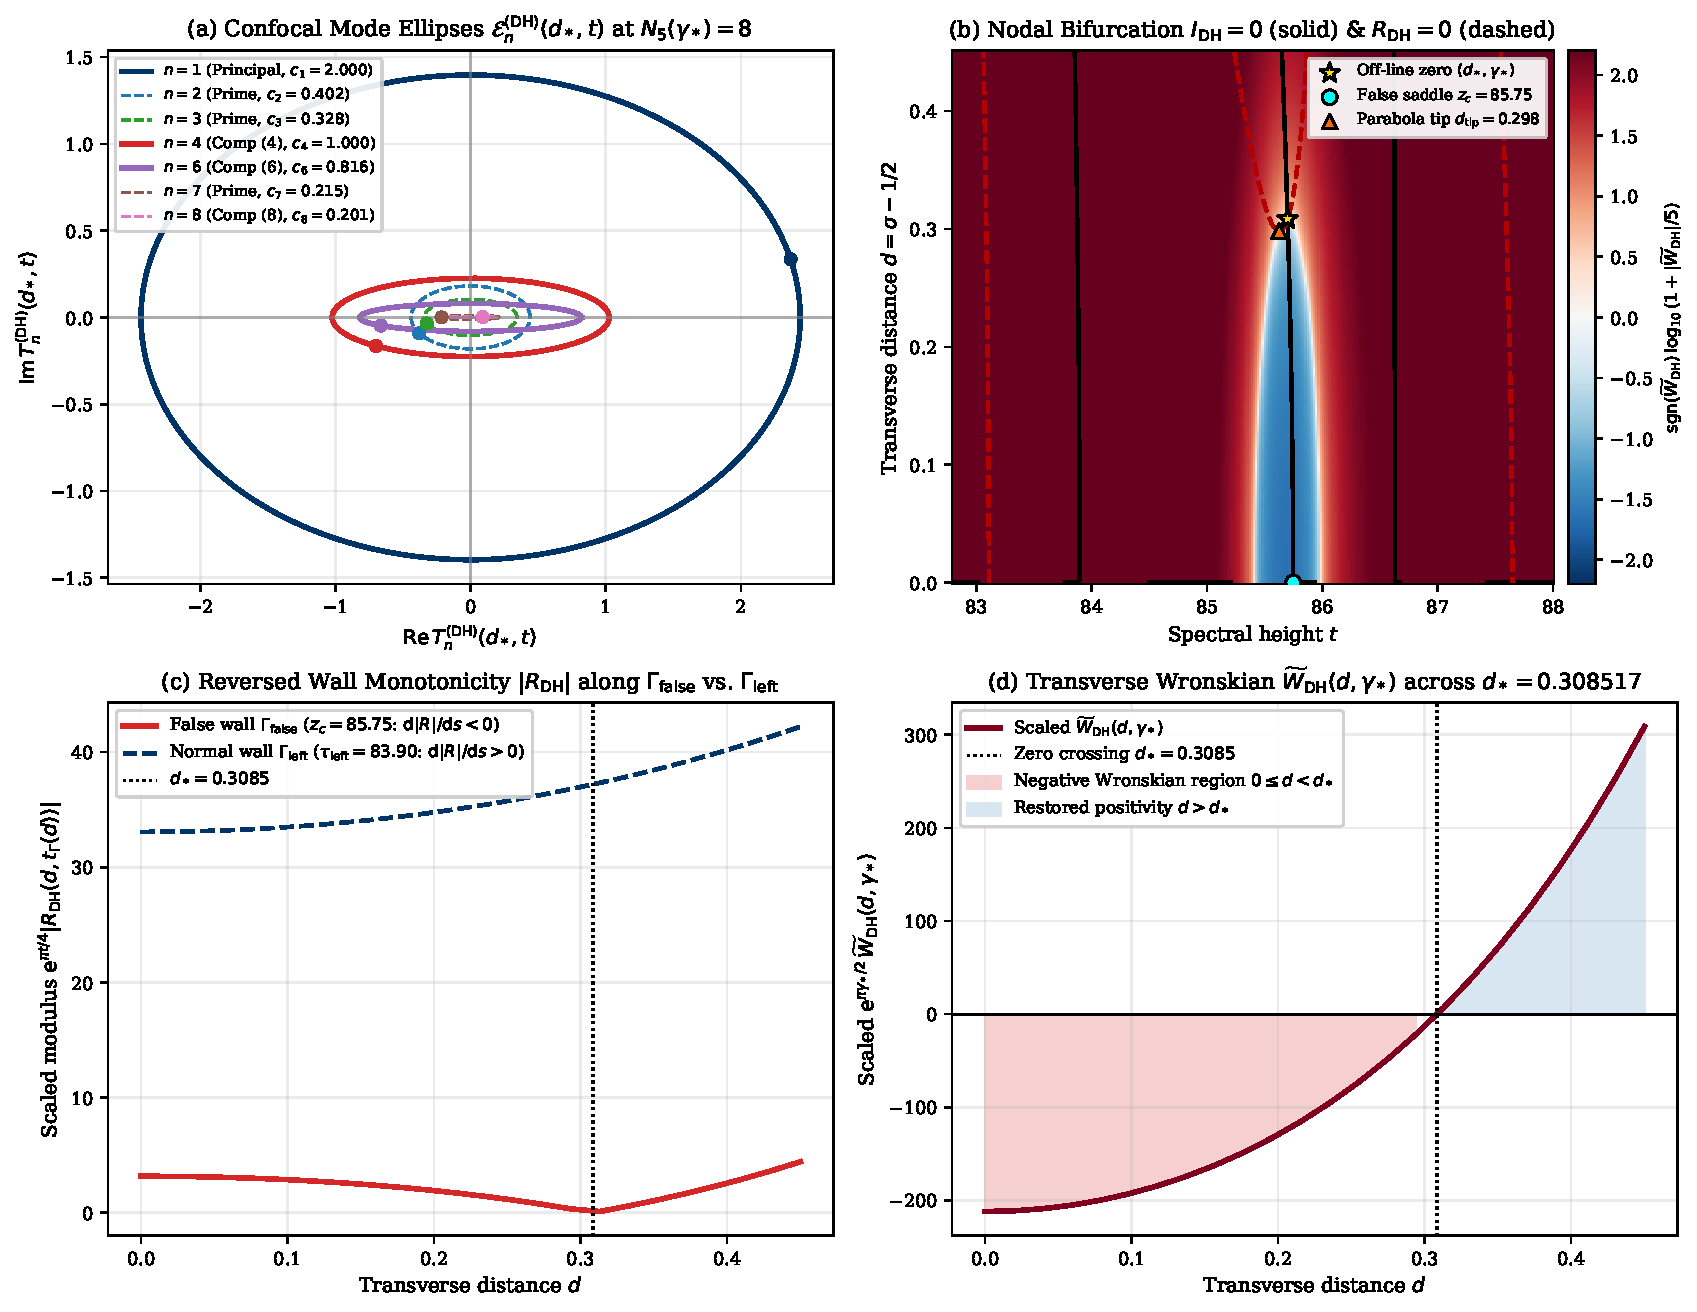
\includegraphics[width=0.98\textwidth]{figures/fig1_davenport_heilbronn_chladni_bifurcation.pdf}
\caption{Davenport--Heilbronn nodal geometry around $(d_*,\gamma_*) = (0.30852, 85.69935)$. \textbf{(a)}~Confocal mode ellipses for $n=1,\dots,8$. \textbf{(b)}~Nodal curves $I_{\mathrm{DH}}=0$ (solid) and detached loop $R_{\mathrm{DH}}=0$ (dashed) meeting at $(d_*,\gamma_*)$ above $z_{\mathrm{c}} = 85.74720$. \textbf{(c)}~Reversed modulus derivative $\dd|R_{\mathrm{DH}}|/\dd s < 0$ along $\Gamma_{\mathrm{false}}$ versus $\dd|R_{\mathrm{DH}}|/\dd s > 0$ along $\Gamma_{\mathrm{left}}$. \textbf{(d)}~Sign change of $\widetilde{W}_{\mathrm{DH}}(d,\gamma_*)$ across $d_*$.}
\label{fig:dh-bifurcation}
\end{figure}

\begin{figure}[htbp]
\centering
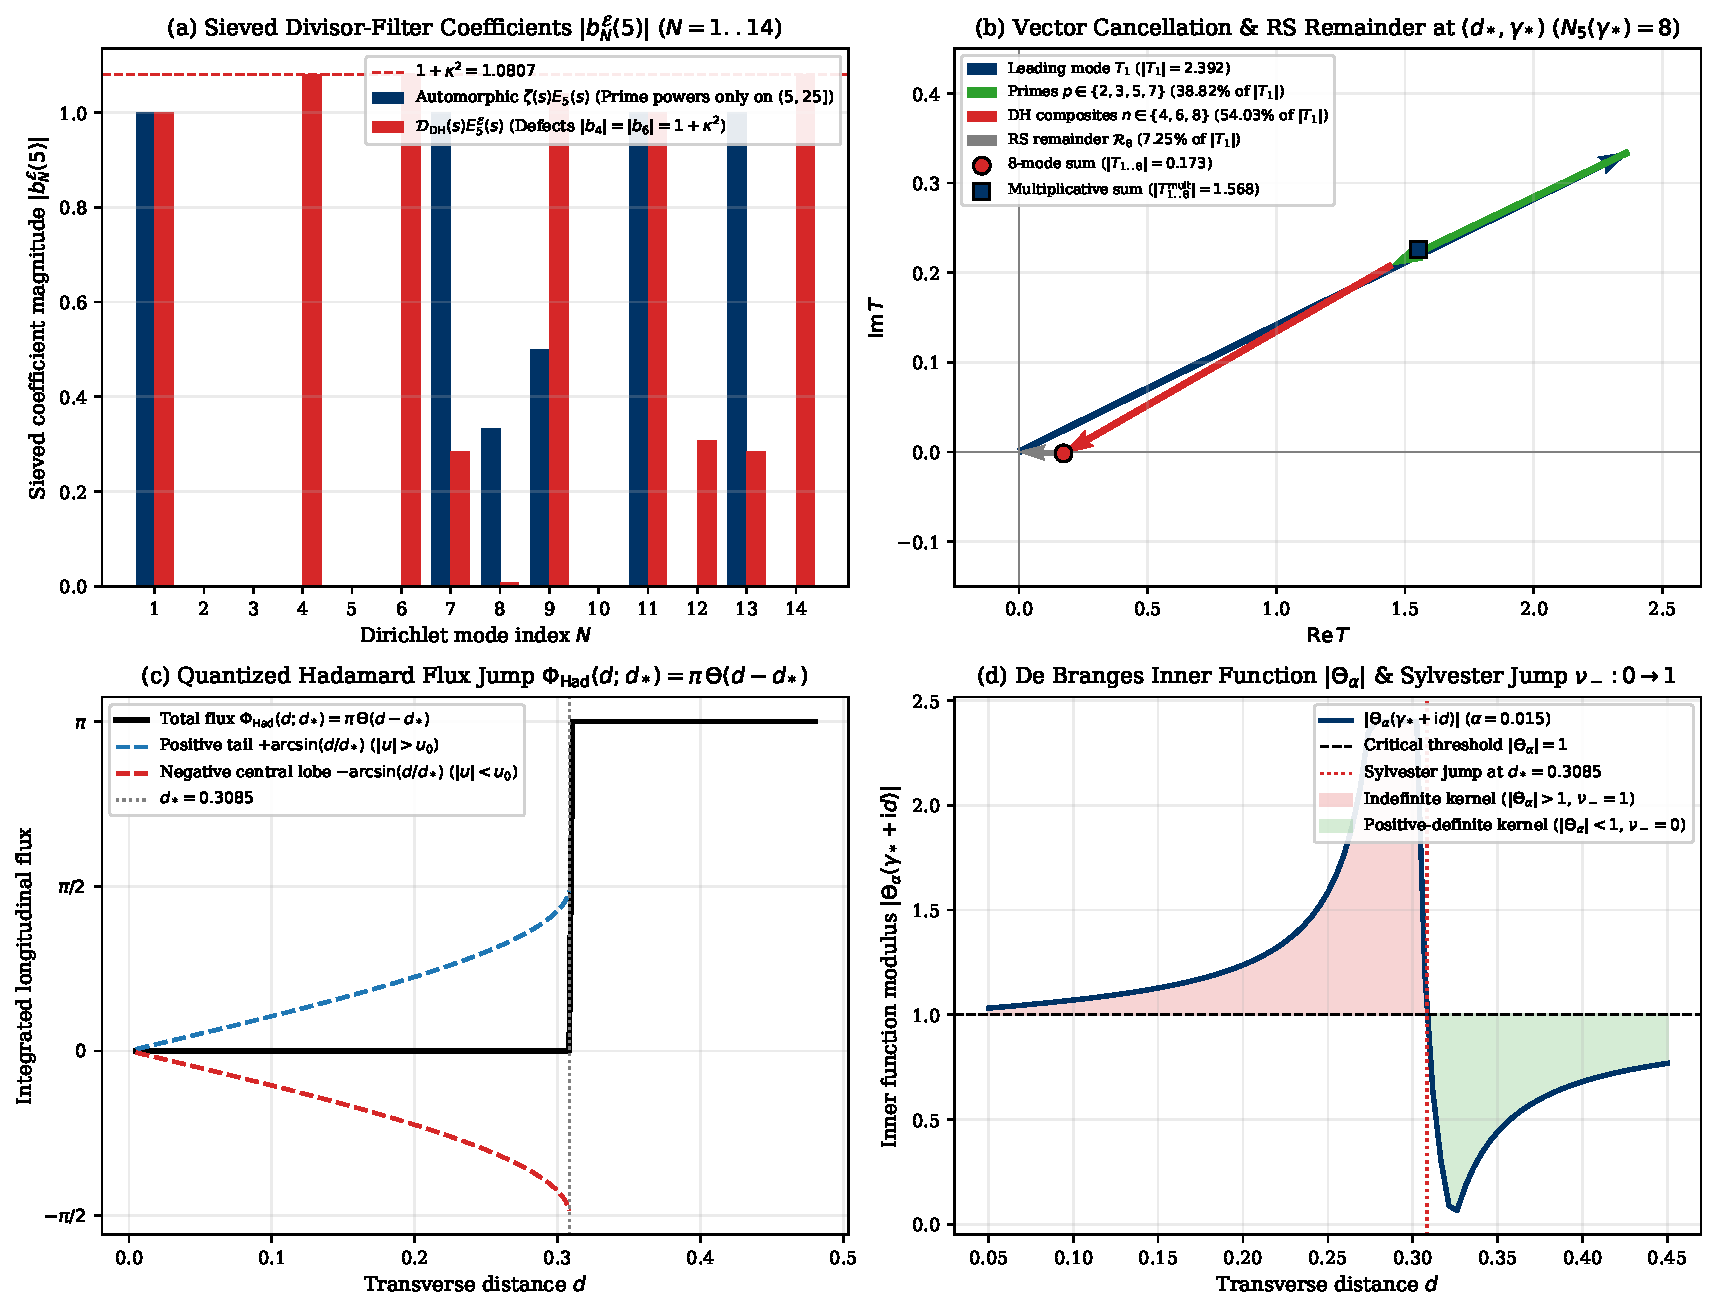
\includegraphics[width=0.98\textwidth]{figures/fig2_prime_gauge_purity_vs_hadamard_flux.pdf}
\caption{Multiplicativity defects and zero-detection profiles. \textbf{(a)}~Sieved coefficients $|b_N^{\mathcal{E}}(5)|$ on $\Reop(s)>1$ for $\zeta(s)$ versus $\mathcal{D}_{\mathrm{DH}}(s)$ ($1+\kappa^2 \approx 1.08070$ defects at $N=4,6,9,14$). \textbf{(b)}~Exact complex vector closure $T_1 + T_{\mathrm{primes}} + T_{\mathrm{comps}} + \mathcal{R}_8 = 0$ at $(d_*,\gamma_*)$, showing the $7.25126\%$ Riemann--Siegel remainder $\mathcal{R}_8$. \textbf{(c)}~Quantized Hadamard step $\pi\,\Theta(d-d_*)$ and $\pm\arcsin(d/d_*)$ lobes. \textbf{(d)}~Modulus $|\Theta_\alpha^{\mathrm{DH}}(\gamma_*+\ii d)|$ and Sylvester jump $\nu_- : 0 \to 1$.}
\label{fig:prime-gauge-flux}
\end{figure}

\section{Scope, limitations, and structural obstructions}
\label{sec:scope}

To prevent overinterpretation of the results proved above, we record four sharp boundaries:
\begin{enumerate}[label=\textup{\arabic*.},leftmargin=2.2em]
  \item \textbf{Detection versus prevention:} Proposition~\ref{prop:fourfold-diagnostics} consists of contrapositives of classical critical-line equivalences \cite{hinkkanen1997,lagarias1999,debranges1968,ariasdereyna2003}. Proving unconditionally that $c_1^\zeta(\tau_k) > 0$, $\widetilde{W}_\zeta(d,t) > 0$, or $\nu_- = 0$ for all heights $t \in \R$ is logically equivalent to the Riemann Hypothesis, not an independent proof of it.
  \item \textbf{Convergence barrier for Euler-product mollifiers:} In Theorem~\ref{thm:prime-gauge-breakdown}(i), while the finite prime-factor polynomial $E_X^{(f)}(s) = \prod_{p\le X} P_p^{(f)}(p^{-s})$ is entire (and preserves all zeros inside $0 < \Reop(s) < 1$ because $1 - \alpha_{p,i}p^{-s}$ vanishes only on $\Reop(s) = \frac{\ln|\alpha_{p,i}|}{\ln p}$), the infinite tail $\prod_{p>X} P_p^{(f)}(p^{-s})^{-1}$ and Dirichlet logarithm $\sum \Lambda_f(n)/(n^s\ln n)$ converge absolutely only on $\Reop(s) > 1$. Inside the critical strip, prime-power sieving leaves oscillatory Dirichlet polynomials coupled to an analytic-continuation remainder whose pointwise phase alignment (the Kronecker--Voronin barrier) remains open.
  \item \textbf{Failure of diagonal-dominance arguments:} Proposition~\ref{prop:confocal-ellipse} proves that single-mode hyperbolic growth $|T_n^{(f)}(d,t)|^2 \ge |T_n^{(f)}(0,t)|^2$ holds identically for $\mathcal{D}_{\mathrm{DH}}(s)$ at $(d_*,\gamma_*)$. Hence diagonal Wronskian positivity never suffices to rule out off-line zeros without controlling all $\binom{N_f(t)}{2}$ off-diagonal cross-terms and the Riemann--Siegel remainder $\mathcal{R}_{N_f(t)}$.
  \item \textbf{Degree $d_f \ge 2$ saddle horizons:} For degree-$d_f$ Selberg-class $L$-functions \cite{selberg1992,kaczorowski1999}, $N_f(t) \asymp t^{d_f/2}$ grows faster with~$t$ when $d_f \ge 2$ (e.g.\ $L(s,\Delta)$), increasing the dimension of the off-diagonal cross-term sum quadratically as $\mathcal{O}(t^{d_f})$.
\end{enumerate}

\appendix

\section{Interval-Arithmetic and Quadrature Protocol}
\label{app:interval}

All numerical quantities in Tables~\ref{tab:branch-damping}--\ref{tab:diagnostics} and Figures~\ref{fig:dh-bifurcation}--\ref{fig:prime-gauge-flux} are generated and audited by the reproducibility suite \nolinkurl{scripts/verify_paper12_selberg_davenport_heilbronn.py}:
\begin{enumerate}[label=(\alph*),leftmargin=2.2em]
  \item \textbf{60-decimal evaluation and root isolation:} $\mathcal{D}_{\mathrm{DH}}(s)$ and $\Xi_{\mathrm{DH}}(z)$ are evaluated to 60~decimal places (\texttt{mp.dps = 60}) via exact Hurwitz zeta decomposition $L(s,\chi_5) = 5^{-s}\sum_{a=1}^{4}\chi_5(a)\zeta(s,a/5)$, isolating $(d_*,\gamma_*)$ and $z_{\mathrm{c}}$ to residuals $|\Xi_{\mathrm{DH}}(\gamma_* - \ii d_*)| < 10^{-58}$ and $|\Xi_{\mathrm{DH}}'(z_{\mathrm{c}})| < 10^{-58}$.
  \item \textbf{35-decimal interval enclosures:} Using \texttt{mpmath.iv} (\texttt{iv.dps = 35}), interval arithmetic certifies $\rho_{\Gamma,f}(d_*,t) < \ee^{-2d_*\vartheta_f'(t)}$, $\delta_{\mathrm{DH}}(m,n) = \pm(1+\kappa^2)$ within width $< 10^{-33}$, and strict negativity $\Xi_{\mathrm{DH}}(t)\Xi_{\mathrm{DH}}''(t) > 0$ ($c_1^{\mathrm{DH}}(t) < 0$) across the enclosure of $z_{\mathrm{c}}$.
  \item \textbf{2D grid visualization:} A $180 \times 280$ grid ($50{,}400$ evaluations on $d \in [0.00000, 0.45000]$, $t \in [82.80000, 88.00000]$) maps the nodal curves $I_{\mathrm{DH}} = 0$, $R_{\mathrm{DH}} = 0$, and $\widetilde{W}_{\mathrm{DH}}(d,t)$ in Figure~\ref{fig:dh-bifurcation} ($2{,}962 / 50{,}400 = 5.87698\%$ negative-Wronskian cells around $(d_*,\gamma_*)$).
\end{enumerate}

\section*{Use of AI and computational verification}

Portions of the symbolic algebra exploration, literature cross-checking, manuscript drafting, and Python verification suite (\nolinkurl{verify_paper12_selberg_davenport_heilbronn.py}) were assisted by Google Gemini. Every mathematical identity, asymptotic condition, citation, and numerical table in this paper was independently checked by symbolic algebra and multi-precision interval computation, and the author assumes full responsibility for the accuracy and scope of all claims.

\begin{thebibliography}{99}

\bibitem{ariasdereyna2003}
J.~Arias~de~Reyna, \emph{X-Ray of Riemann zeta-function}, preprint (2003), \texttt{arXiv:math/0309433}.

\bibitem{balanzario2007}
E.~P.~Balanzario and J.~S\'anchez-Ortiz, \emph{Zeros of the Davenport--Heilbronn counterexample}, Math. Comp. \textbf{76} (2007), no.~260, 2045--2049.

\bibitem{bombieri2011}
E.~Bombieri and A.~Ghosh, \emph{Around the Davenport--Heilbronn function}, Russian Math. Surveys \textbf{66} (2011), no.~2, 221--270.

\bibitem{csordas1994}
G.~Csordas, W.~Smith, and R.~S.~Varga, \emph{Lehmer pairs of zeros, the de~Bruijn--Newman constant $\Lambda$, and the Riemann Hypothesis}, Constr. Approx. \textbf{10} (1994), no.~1, 107--129.

\bibitem{davenport1936}
H.~Davenport and H.~Heilbronn, \emph{On the zeros of certain Dirichlet series I, II}, J. London Math. Soc. \textbf{11} (1936), 181--185, 307--312.

\bibitem{debranges1968}
L.~de~Branges, \emph{Hilbert Spaces of Entire Functions}, Prentice-Hall, Englewood Cliffs, NJ, 1968.

\bibitem{gonek2007}
S.~M.~Gonek, C.~P.~Hughes, and J.~P.~Keating, \emph{A hybrid Euler--Hadamard product for the Riemann zeta function}, Duke Math. J. \textbf{136} (2007), no.~3, 507--549.

\bibitem{hecke1936}
E.~Hecke, \emph{\"Uber die Bestimmung Dirichletscher Reihen durch ihre Funktionalgleichung}, Math. Ann. \textbf{112} (1936), 664--699.

\bibitem{hinkkanen1997}
A.~Hinkkanen, \emph{On functions of bounded type}, Complex Variables Theory Appl. \textbf{34} (1997), no.~1--2, 119--139.

\bibitem{hudson1974}
R.~L.~Hudson, \emph{When is the Wigner quasi-probability density non-negative?}, Rep. Math. Phys. \textbf{6} (1974), no.~2, 249--252.

\bibitem{iwaniec2004}
H.~Iwaniec and E.~Kowalski, \emph{Analytic Number Theory}, Amer. Math. Soc. Colloq. Publ., vol.~53, Amer. Math. Soc., Providence, RI, 2004.

\bibitem{jensen1913}
J.~L.~W.~V.~Jensen, \emph{Recherches sur la th\'eorie des \'equations}, Acta Math. \textbf{36} (1913), no.~1, 181--195.

\bibitem{kaczorowski1999}
J.~Kaczorowski and A.~Perelli, \emph{On the structure of the Selberg class, I: $0 \le d \le 1$}, Acta Math. \textbf{182} (1999), no.~2, 207--241.

\bibitem{lagarias1999}
J.~C.~Lagarias, \emph{On a positivity property of the Riemann $\xi$-function}, Acta Arith. \textbf{89} (1999), no.~3, 217--234.

\bibitem{polya1926}
G.~P\'olya, \emph{Bemerkung \"uber die Integraldarstellung der Riemannschen $\xi$-Funktion}, Acta Math. \textbf{48} (1926), 305--317.

\bibitem{riemann1859}
B.~Riemann, \emph{Ueber die Anzahl der Primzahlen unter einer gegebenen Gr\"osse}, Monatsber. K\"onigl. Preuss. Akad. Wiss. Berlin (1859), 671--680.

\bibitem{selberg1992}
A.~Selberg, \emph{Old and new conjectures and results about a class of Dirichlet series}, in Proceedings of the Amalfi Conference on Analytic Number Theory (Maiori, 1989), Univ. Salerno, 1992, pp.~367--385.

\bibitem{speiser1934}
A.~Speiser, \emph{Geometrisches zur Riemannschen Zetafunktion}, Math. Ann. \textbf{110} (1934), 514--521.

\bibitem{spira1994}
R.~Spira, \emph{Some zeros of the Titchmarsh counterexample}, Math. Comp. \textbf{63} (1994), no.~208, 747--748.

\bibitem{titchmarsh1986}
E.~C.~Titchmarsh, \emph{The Theory of the Riemann Zeta-Function}, 2nd ed., revised by D.~R.~Heath-Brown, Oxford Univ. Press, Oxford, 1986.

\bibitem{wigner1932}
E.~Wigner, \emph{On the quantum correction for thermodynamic equilibrium}, Phys. Rev. \textbf{40} (1932), 749--759.

\end{thebibliography}

\end{document}
